\documentclass[12pt,a4paper]{book}
\usepackage[T5]{fontenc}
\usepackage[utf8]{inputenc}
\usepackage[vietnamese]{babel}
\usepackage{amsmath, amssymb}
\usepackage{enumerate}
\usepackage{geometry}
\usepackage{graphicx}
\usepackage{caption}
\usepackage[most]{tcolorbox}

\geometry{margin=1in}

\newenvironment{problem}[1][]{
  \par\noindent\textbf{Bài #1.}\ \ignorespaces
}{\par}

\begin{document}

\chapter{Tính chất của số học}
\section{Vì sao bắt đầu bằng số học?}

Con đã biết cộng, trừ, nhân, chia. Thậm chí con còn có thể giải
được nhiều bài trong chương này rồi. Vậy tại sao chúng ta lại mở
đầu cuốn sách bằng \emph{cả một chương} nói về số học?

Để trả lời, ta quay lại tên sách: \emph{Tiền đại số}. \emph{Tiền
đại số} là gì? Có nhiều cách hiểu khác nhau, nhưng chúng mình
(những người viết sách) xem \emph{tiền đại số} là chiếc cầu nối
giữa \emph{số học} và \emph{đại số}.

\emph{Số học} là những điều căn bản: cộng, trừ, nhân, chia, và có
thể thêm vài điều thú vị như bình phương hay căn bậc hai. Có lẽ
con đã học phần lớn những điều này rồi. Điều thường làm con thấy
khó nhất trong số học là \emph{bài toán bằng lời}, ví dụ: “Lan có
$5$ quả táo, Minh có $7$ quả, hỏi cả hai bạn có tất cả bao nhiêu
quả?” Khi lớn hơn, các số có thể to hơn, nhưng kiểu bài thì không
khó hơn bao nhiêu. Số học rất giỏi khi giải những việc đơn giản
như đếm đồ vật. 

Nhưng khi bài toán trở nên \emph{phức tạp} hơn — như tính đường
bay của tên lửa, phân tích thị trường tiền tệ, hay đếm xem có bao
nhiêu cách để một tin nhắn đi qua các trạm thu phát — ta cần một
“hộp dụng cụ” mạnh mẽ hơn.

“Hộp dụng cụ” đó là \emph{đại số}. Đại số là ngôn ngữ của toán
học nâng cao. Đại số cho ta những công cụ để lấy ý tưởng từ số học
và biến chúng thành các quy tắc \emph{khái quát}, nghĩa là ta có
thể dùng các ý tưởng ấy không chỉ cho bài toán số học, mà còn cho
rất nhiều dạng bài khác nữa.

\section{Ví dụ về tính chất của số học}

Ta hãy xem một ví dụ đơn giản. Dùng số học, ta có thể chứng minh rằng:
\[
2\times(3+5)=(2\times3)+(2\times5).
\]
Vì vế trái là $2\times8=16$, còn vế phải là $6+10=16$. Hai bên bằng nhau.

Nhưng đại số cho ta một quy tắc tổng quát hơn:
\[
a\times(b+c)=(a\times b)+(a\times c),
\]
đúng với mọi số $a,b,c$. Trong toán học cao hơn, $a,b,c$ có thể không
chỉ là các số quen thuộc, mà có thể là những đối tượng toán học phức
tạp hơn. (Và khi đó, dấu “$+$” hay “$\times$” có thể mang ý nghĩa khác
với phép cộng và phép nhân thông thường — nhưng điều đó ta sẽ học sau.)

Mục tiêu ban đầu trong chương này là đặt ra những quy tắc cơ bản của
số học, và giúp con hiểu \emph{vì sao} chúng lại đúng. Khi nắm được
các quy tắc ấy, con sẽ sẵn sàng bắt đầu tư duy theo hướng đại số.

\subsection*{Vì sao cần hiểu “vì sao”?}
Khi đọc đến đây, con đã đủ lớn để không chỉ biết \emph{làm thế nào}
để tính, mà còn muốn biết \emph{vì sao} cách tính đó lại đúng. Hiểu
vì sao toán học hoạt động như thế là chìa khóa để giải được các bài
toán khó hơn. Nếu con chỉ biết cách bấm máy hoặc làm theo công thức mà
không hiểu bản chất, thì khi gặp bài khác lạ, con sẽ rất khó sửa đổi
hay mở rộng cách làm đó. Vì vậy, trong cuốn sách này, thầy cô sẽ không
chỉ nói “làm thế này để ra kết quả”, mà sẽ luôn cố gắng chỉ ra “vì sao
nó đúng”.

\subsection*{Kết thúc chương này, con sẽ biết giải thích vì sao:}
\begin{itemize}
  \item $(-5)\times(-7)=35$ (và không phải $-35$).
  \item $(1990\times1991)-(1989\times1990)=3980$ (và có thể nhẩm được!).
  \item $8\div\tfrac{1}{7}=56$.
  \item $(4\times10\times49)\div(2\times5\times7)=28$ (cũng nhẩm được!).
\end{itemize}

Con sẽ hiểu tất cả những điều này không phải vì học thuộc lòng công
thức, mà vì hiểu được toán học ẩn bên trong các phép tính đó.

\subsection*{Một chút lưu ý}
Đôi khi, các nhà toán học ở những nơi khác nhau dùng từ hơi khác nhau
cho cùng một ý. Giống như người Mỹ gọi là “truck” còn người Anh gọi là
“lorry”, nhưng cùng chỉ chiếc xe tải. Vì thế, trước khi học tiếp, ta
sẽ thống nhất một số từ để dùng trong cuốn sách này cho rõ ràng nhé.

\section{Đường số và các loại số}

Hình dưới là \emph{đường số}. Đường số kéo dài mãi về hai phía.
Mỗi vạch nhỏ chỉ một \emph{số nguyên}. Ta thấy các số
\[
\ldots,-6,-5,-4,-3,-2,-1,0,1,2,3,4,5,6,\ldots
\]

\begin{figure}[ht!]
  \centering
  % Dùng bản PDF khi biên dịch LaTeX
  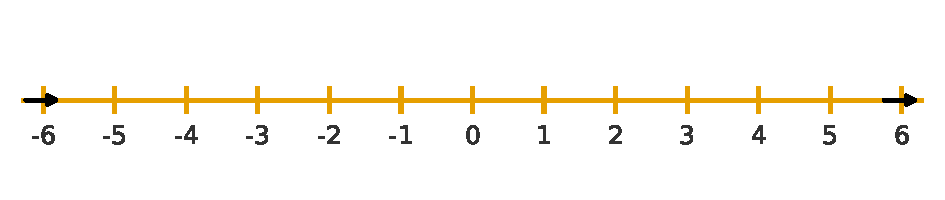
\includegraphics[width=0.9\textwidth]{img/fig-numberline.pdf}
  \caption*{\small Đường số với các vạch từ $-6$ đến $6$ và mũi tên chỉ rằng
  đường số còn kéo dài nữa.}
\end{figure}

\noindent\textbf{Tên gọi đơn giản:}
\begin{itemize}
  \item \textit{Số dương}: đứng bên phải $0$.
  \item \textit{Số âm}: đứng bên trái $0$.
  \item \textit{Không âm}: là số dương hoặc $0$.
  \item \textit{Không dương}: là số âm hoặc $0$.
  \item \textit{Khác $0$}: mọi số trừ $0$.
\end{itemize}

\begin{quote}
\textbf{Ghi chú:} Có nơi gọi \emph{số tự nhiên} là $1,2,3,\ldots$,
có nơi tính cả $0$. Trong tài liệu này, ta dùng: \emph{số nguyên dương}
cho $1,2,3,\ldots$ và \emph{số nguyên không âm} cho $0,1,2,\ldots$.
\end{quote}


\section{Phép cộng}

Ta bắt đầu với phép toán quen thuộc nhất: \emph{phép cộng}.
Tuy đơn giản, nhưng hiểu rõ tính chất của phép cộng sẽ giúp con
tính nhẩm nhanh và làm chủ các phép tính phức tạp hơn.

\begin{problem}[1.1]
Dựa vào \emph{hai hình vẽ} bên dưới, hãy giải thích vì sao
$2+3=3+2$.

\begin{figure}[h!]
  \centering
  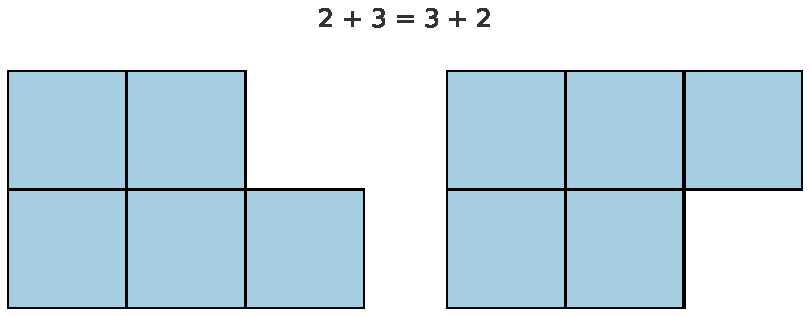
\includegraphics[width=0.55\textwidth]{img/fig-prob1.1.pdf}
  \caption*{\small Gợi ý: đổi chỗ hai nhóm ô vuông, tổng vẫn không đổi.}
\end{figure}
\end{problem}

\begin{problem}[1.2]
Dựa vào \emph{hai hình vẽ} bên dưới, hãy giải thích vì sao
$(2+3)+4=2+(3+4)$.

\begin{figure}[h!]
  \centering
  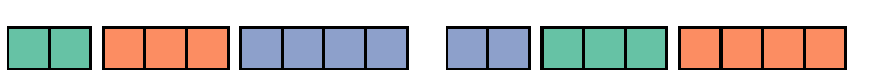
\includegraphics[width=0.55\textwidth]{img/fig-prob1.2.pdf}
  \caption*{\small Gợi ý: cộng nhóm đầu tiên hay nhóm sau đều cho cùng tổng.}
\end{figure}
\end{problem}

\begin{problem}[1.3]
\begin{enumerate}[(a)]
  \item Dùng các tính chất ở trên, giải thích:
  \[
  472+(219+28)=(472+28)+219.
  \]
  \item Tính nhẩm $472+(219+28)$.
  \begin{flushright}\small(Nguồn: MATHCOUNTS)\end{flushright}
\end{enumerate}
\end{problem}

\begin{problem}[1.4]
Tính:
\[
(2+12+22+32)+(8+18+28+38).
\]
\begin{flushright}\small(Nguồn: MATHCOUNTS)\end{flushright}
\end{problem}

\begin{problem}[1.5]
Tính tổng:
\[
1+2+3+\cdots+19+20.
\]
\textit{Gợi ý:} Dấu \texttt{$\cdots$} nghĩa là ta cộng tất cả số theo
mẫu từ $1$ đến $20$.
\end{problem}


\begin{problem}[1.6]
Dựa vào hình dưới đây, hãy giải thích vì sao $2 + 0 = 2$.

\begin{figure}[h!]
  \centering
  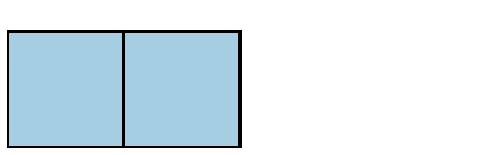
\includegraphics[width=0.55\textwidth]{img/fig-prob1.6.pdf}
  \caption*{\small Hai ô vuông cộng với “không ô vuông” vẫn bằng hai ô vuông.}
\end{figure}
\end{problem}

\begin{problem}[1.1]
Dựa vào hai hình bên dưới, hãy giải thích vì sao $2 + 3 = 3 + 2$.

\begin{figure}[h!]
  \centering
  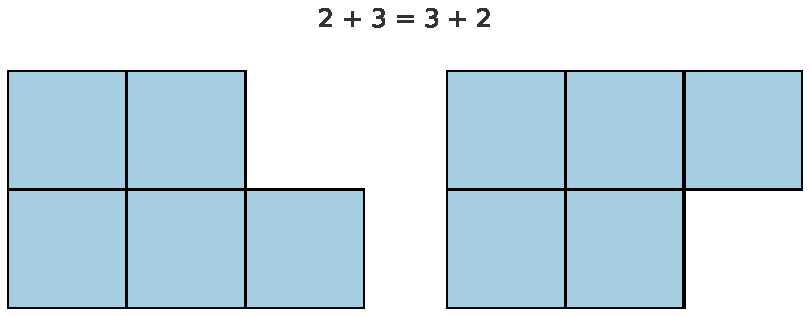
\includegraphics[width=0.55\textwidth]{img/fig-prob1.1.pdf}
  \caption*{\small Hai cách sắp xếp khác nhau của cùng số ô vuông.}
\end{figure}

\textbf{Lời giải:}  
Trước hết, hãy nhìn vào hình bên trái. Hàng đầu tiên có $2$ ô vuông, hàng thứ hai có $3$ ô vuông.  
Tổng cộng là $2 + 3$ ô vuông.  

Bây giờ, nhìn sang hình bên phải. Hàng đầu tiên có $3$ ô vuông, hàng thứ hai có $2$ ô vuông.  
Tổng cộng cũng là $3 + 2$ ô vuông.  

Hình bên phải thực ra chỉ là bản lật ngược của hình bên trái.  
Lật ngược hình không làm thay đổi số lượng ô vuông.  
Do đó, ta kết luận rằng:
\[
2 + 3 = 3 + 2.
\]
\end{problem}

Mỗi khi chúng ta cộng hai số, \textbf{thứ tự} của các số không làm thay đổi kết quả.  
Ví dụ:
\[
5 + 17 = 17 + 5, \quad 32 + 999 = 999 + 32.
\]
Có vô số ví dụ như vậy.  
Tất nhiên, ta không thể viết hết ra được, nên ta dùng cách viết tổng quát hơn:
\[
\text{số thứ nhất} + \text{số thứ hai} = \text{số thứ hai} + \text{số thứ nhất.}
\]

Để ngắn gọn, ta gọi số thứ nhất là $a$, số thứ hai là $b$.  
Khi đó, ta có:
\[
a + b = b + a.
\]

Ở đây, $a$ và $b$ có thể là bất kỳ số nào (hoặc có thể bằng nhau).  
Ví dụ, nếu $a = 2$ và $b = 3$, ta có $2 + 3 = 3 + 2$.  
Nếu $a = 100$ và $b = 200$, ta có $100 + 200 = 200 + 100$.  

Chữ $a$ và $b$ được gọi là \emph{biến} (hay \emph{ẩn}), vì giá trị của chúng có thể thay đổi tuỳ từng bài toán.

\begin{quote}
\textbf{Tính chất giao hoán của phép cộng:}  
Với mọi số $a$ và $b$, ta luôn có
\[
a + b = b + a.
\]
\end{quote}

Trong Bài 1.1, ta đã thấy $a + b = b + a$ là đúng khi $a = 2$, $b = 3$.  
Nhưng một ví dụ riêng lẻ chưa đủ để chứng minh rằng công thức này đúng với \emph{mọi} số $a$ và $b$.  
Để làm được điều đó, ta sẽ học thêm nhiều bước lập luận chặt chẽ hơn ở các chương sau.

Bây giờ ta đã hiểu rằng thứ tự của hai số khi cộng không làm thay đổi kết quả.
Vậy nếu ta cộng \emph{ba} số thì sao?

\begin{problem}[1.2]
Dựa vào hai hình dưới đây, hãy giải thích vì sao
\[
(2 + 3) + 4 = 2 + (3 + 4).
\]

\begin{figure}[h!]
  \centering
  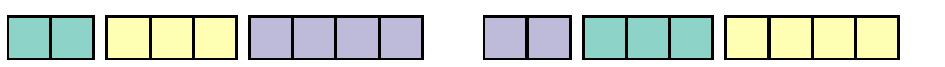
\includegraphics[width=0.75\textwidth]{img/fig-prob1.2-assoc.pdf}
  \caption*{\small Hai cách nhóm khác nhau của ba nhóm ô vuông.}
\end{figure}
\end{problem}

\noindent\textbf{Gợi ý:} Dấu ngoặc cho biết ta cần tính phần nào trước.
Ví dụ, $(3 + 4) \times 5$ nghĩa là $7 \times 5$, trong khi $(4 \times 5)$ nghĩa là $3 + 20$.


\textbf{Lời giải cho Bài 1.2:}  
Với mỗi hình, ta sẽ đếm số ô vuông sáng, rồi đếm số ô vuông tối, sau đó cộng hai kết quả lại.

- Trong hình bên trái: có $(2 + 3)$ ô sáng và $4$ ô tối.  
  Tổng cộng có $(2 + 3) + 4$ ô vuông.

- Trong hình bên phải: có $2$ ô sáng và $(3 + 4)$ ô tối.  
  Tổng cộng có $2 + (3 + 4)$ ô vuông.

Điểm khác nhau duy nhất giữa hai hình là màu của hàng ở giữa.  
Việc đổi màu không làm thay đổi số ô, nên ta kết luận:
\[
(2 + 3) + 4 = 2 + (3 + 4).
\]

Từ đây, ta có thể viết quy tắc tương tự cho bất kỳ ba số nào:
\[
(a + b) + c = a + (b + c).
\]
Nói cách khác, nếu ta cộng $a$ và $b$ trước rồi cộng $c$,  
hay cộng $b$ và $c$ trước rồi cộng $a$, thì kết quả vẫn như nhau.  
Tính chất này gọi là \textbf{tính chất kết hợp của phép cộng.}

\begin{quote}
\textbf{Tính chất kết hợp của phép cộng:}  
Với mọi số $a, b, c$, ta luôn có:
\[
(a + b) + c = a + (b + c).
\]
\end{quote}

\begin{tcolorbox}[colback=yellow!10!white,colframe=orange!80!black,title={Lưu ý quan trọng}]
Học sinh đôi khi nhầm giữa hai tính chất “\emph{giao hoán}” và “\emph{kết hợp}”.  
Trong \textbf{tính chất giao hoán}, ta \emph{đổi chỗ} các số (ví dụ $a+b=b+a$).  
Trong \textbf{tính chất kết hợp}, ta \emph{nhóm} các số khác nhau  
(ví dụ $(a+b)+c=a+(b+c)$), nhưng không đổi vị trí của chúng.
\end{tcolorbox}

%----------------------------------------
% 1.3  Quy tắc đổi chỗ + kết hợp giúp cộng theo "bất kỳ thứ tự"
%----------------------------------------

\paragraph{Gộp lại,} hai tính chất \emph{giao hoán} và \emph{kết hợp}
mạnh mẽ hơn ta tưởng. Chúng cho phép ta cộng một dãy số theo \emph{bất
kỳ thứ tự} nào. Bài tiếp theo minh hoạ nguyên tắc “cộng theo mọi thứ
tự” này.

\begin{problem}[1.3]
\begin{enumerate}[(a)]
  \item Dùng các tính chất ở Bài 1.1 và 1.2, hãy giải thích vì sao
  \[
    472 + (219 + 28) \;=\; (472 + 28) + 219.
  \]
  \item Tính tổng \(\;472 + (219 + 28)\).
  \begin{flushright}\small(Nguồn: MATHCOUNTS)\end{flushright}
\end{enumerate}
\end{problem}

\noindent\textbf{Lời giải cho Bài 1.3:}

\smallskip
\noindent(a)\; Ta bắt đầu từ vế trái:
\[
  472 + (219 + 28).
\]
Ta muốn biến đổi để nó trông giống vế phải. Trước hết, ta \emph{đổi
chỗ} \(219\) và \(28\) ở trong ngoặc nhờ tính chất giao hoán, tức là
thay \((219+28)\) bởi lượng bằng nó là \((28+219)\):
\[
  472 + (219 + 28) \;=\; 472 + (28 + 219).
\]
Biểu thức này đã gần giống điều ta cần: \((472 + 28) + 219\).
Thực ra hai biểu thức đó \emph{bằng nhau} nhờ tính chất kết hợp, vì ta
được phép \emph{đổi cách nhóm} các số hạng:
\[
\begin{aligned}
  472 + (219 + 28) 
  &= 472 + (28 + 219) && \text{(giao hoán)}\\
  &= (472 + 28) + 219 && \text{(kết hợp).}
\end{aligned}
\]

\smallskip
\noindent(b)\; Từ phần (a), hai biểu thức
\(472 + (219 + 28)\) và \((472 + 28) + 219\) là bằng nhau, nên ta có
thể tính \((472 + 28) + 219\) thay vì tính trực tiếp.
Nhẩm \(472 + 28 = 500\). Vậy ta còn lại \(500 + 219\),
nên kết quả là \(719\).

\medskip
\noindent\(\square\)

\medskip
\noindent\textbf{Điều quan trọng của Bài 1.3:} Ta có thể \emph{sắp xếp
lại} các số trong phép cộng để phép tính trở nên \emph{dễ} hơn. Thường
thì thuận tiện nhất là ghép những số “đẹp” với nhau trước (ví dụ làm
tròn trăm), rồi mới cộng phần còn lại. Trong thực hành, ta sẽ không
viết lại toàn bộ các bước như ở Bài 1.3 mỗi lần. Thay vào đó, ta vận
dụng hiểu biết về \emph{tính chất giao hoán} và \emph{tính chất kết
hợp} để tự do sắp xếp, nhóm lại các số theo cách tốt nhất. Hãy áp dụng
nguyên tắc này cho bài tiếp theo nhé!

%----------------------------------------
% 1.4  Ghép cặp để tính nhanh hơn
%----------------------------------------
\begin{problem}[1.4]
Tính:
\[
(2 + 12 + 22 + 32) + (8 + 18 + 28 + 38).
\]
\begin{flushright}\small(Nguồn: MATHCOUNTS)\end{flushright}
\end{problem}

\noindent\textbf{Lời giải cho Bài 1.4:}  
Ta có thể bắt đầu cộng từng số, nhưng như vậy sẽ mất nhiều thời gian.  
Thay vào đó, hãy sắp xếp lại các số sao cho mỗi cặp có cùng tổng.  
Cụ thể, ta ghép mỗi số ở nhóm thứ nhất với một số ở nhóm thứ hai như sau:
\[
(2 + 38) + (12 + 28) + (22 + 18) + (32 + 8).
\]
Mỗi cặp đều có tổng bằng \(40\).  
Vì có bốn cặp, nên tổng bằng:
\[
40 + 40 + 40 + 40 = 160.
\]
Vậy kết quả là \(\boxed{160}.\)
\medskip

---

%----------------------------------------
% 1.5  Cộng dãy số dài bằng cách ghép cặp
%----------------------------------------
\begin{problem}[1.5]
Tính tổng:
\[
1 + 2 + 3 + \cdots + 19 + 20.
\]
\textit{Gợi ý:} Dấu \texttt{$\cdots$} nghĩa là ta cộng tất cả các số theo mẫu,  
nên ở đây ta cộng các số nguyên dương từ 1 đến 20.
\end{problem}

\noindent\textbf{Lời giải cho Bài 1.5:}  
Chúng ta chắc chắn không muốn cộng lần lượt 20 số đâu!  
Hãy thử ghép các số thành cặp để mỗi cặp có cùng tổng.  
Ta ghép số nhỏ nhất với số lớn nhất, số nhỏ thứ hai với số lớn thứ hai, v.v.:
\[
(1 + 20) + (2 + 19) + (3 + 18) + \cdots + (10 + 11).
\]
Ta có 20 số, tức là 10 cặp.  
Mỗi cặp đều bằng \(21\).  
Vậy tổng là:
\[
21 + 21 + 21 + 21 + 21 + 21 + 21 + 21 + 21 + 21.
\]
Cộng 10 lần 21 tức là \(10 \times 21 = 210.\)
\[
\boxed{210}.
\]

---

%----------------------------------------
% 1.6  Cộng thêm số 0
%----------------------------------------
\begin{problem}[1.6]
Dựa vào hình dưới đây, hãy giải thích vì sao \(2 + 0 = 2.\)

\begin{figure}[h!]
  \centering
  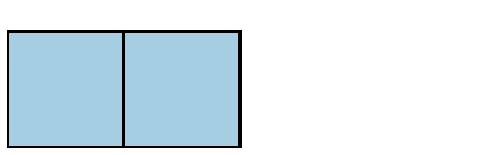
\includegraphics[width=0.4\textwidth]{img/fig-prob1.6.pdf}
  \caption*{\small Hai ô vuông cộng với “không ô vuông” vẫn là hai ô vuông.}
\end{figure}
\end{problem}

\noindent\textbf{Lời giải cho Bài 1.6:}  
Một mặt, ta có 2 ô vuông.  
Mặt khác, có thể nói rằng ta có 2 ô sáng và 0 ô tối.  
Vì vậy ta được phương trình:
\[
2 + 0 = 2.
\]
Khi cộng thêm số 0 vào bất kỳ số nào, kết quả vẫn không thay đổi.

\begin{tcolorbox}[colback=yellow!10!white, colframe=orange!80!black,
title={Tính chất cộng với số không}]
Nếu \(a\) là một số bất kỳ, thì:
\[
a + 0 = a.
\]
\end{tcolorbox}

\end{document}
